%Part of/Parte di https://github.com/f-dinucci/appuntiMeccanicaFluidi/
%License/Licenza Creative Commons Attribution-ShareAlike 4.0 International (CC BY-SA 4.0) - attribution/attribuzione Francesco Di Nucci
%See also/Vedere anche https://creativecommons.org/licenses/by-sa/4.0/ and/e https://creativecommons.org/licenses/by-sa/4.0/legalcode
%
\section{Forze e sforzi}
\subsection{Forze a distanza}
Si può avere una variazione della quantità di moto in un volume di controllo sia per un passaggio di fluido attraverso le superfici che lo delimitano sia per l'azione di una forza a distanza.
%
	\begin{figure}[ht]
		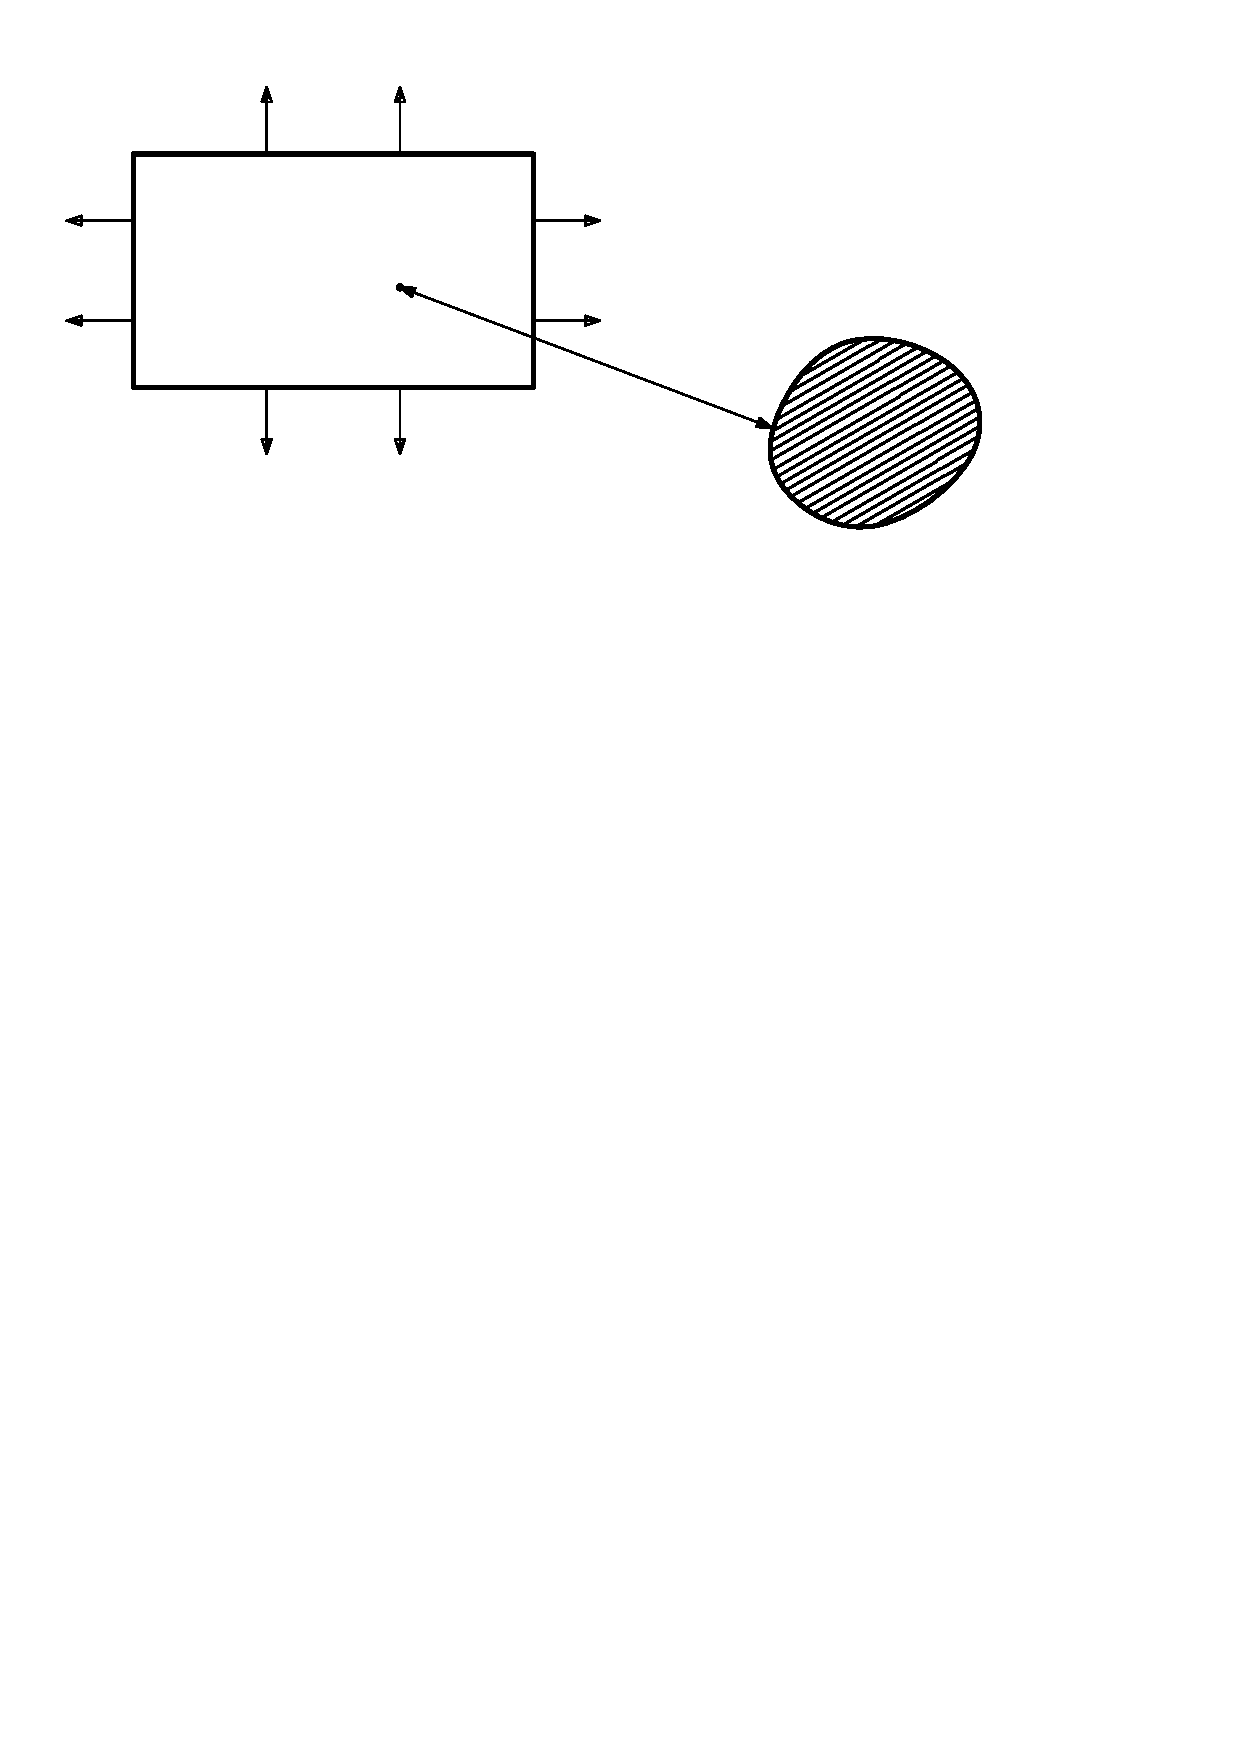
\includegraphics[scale=0.7]{./1.5 Forze e sforzi/1.5-1}
		\centering
		\caption{Esempio di forza a distanza}
	\end{figure}
%
Forze a distanza possono essere ad esempio una forza tra un punto del volume di controllo ed un corpo solido esterno (come la gravità) o ad esempio forze elettriche/magnetiche su di un fluido conduttore.

In termini matematici, dato che le forze a distanza si calcolano tramite un integrale di volume (non di lunghezza), si ha:
	\begin{equation*}
		\begin{gathered}
			\dv{t} \int{q_i \dd{V}} + \oint{J_{Qij} n_j \dd{S}} = \int{f_i \dd{V}} \\
			\text{che in notazione vettoriale è} \\
			\dv{t} \int{\uline{q} \dd{V}} + \oint{\uuline{J}_Q \vdot \uline{n} \dd{S}} = \int{\uline{f} \dd{V}}
		\end{gathered}
	\end{equation*}
Si è quindi definito un prodotto scalare tensore/vettore: 
	\begin{equation*}
		{\qty[\uuline{J}_Q \vdot \uline{n}]}_i = \sum_{i = 1}^{3} {J_{Qij} n_j}
	\end{equation*}
Matematicamente è equivalente ad un prodotto matrice/vettore, scrivere gli indici serve solo ad evidenziare che c'è un sistema di riferimento.

Il prodotto scalare non è commutativo, ma in caso di simmetria (dopo la scelta di un opportuno sistema di riferimento) si ha che si ha che $J_{Qij} = J_{Qji}$, quindi valgono le seguenti:
	\begin{equation*}
		\begin{aligned}
			{\qty[\uuline{J}_Q \vdot \uline{n}]}_i = \sum_{j = 1}^{3} {J_{Qij} n_j} \\
			{\qty[\uline{n} \vdot \uuline{J}_Q]}_i = \sum_{j = 1}^{3} {J_{Qji} n_j}
		\end{aligned}
	\end{equation*}
Questo non è valido sempre, ma si può applicare alla maggior parte dei casi.
%
\subsection{Tensore degli sforzi}
Si consideri un volume di controllo suddiviso in due parti.
%
	\begin{figure}[h]
		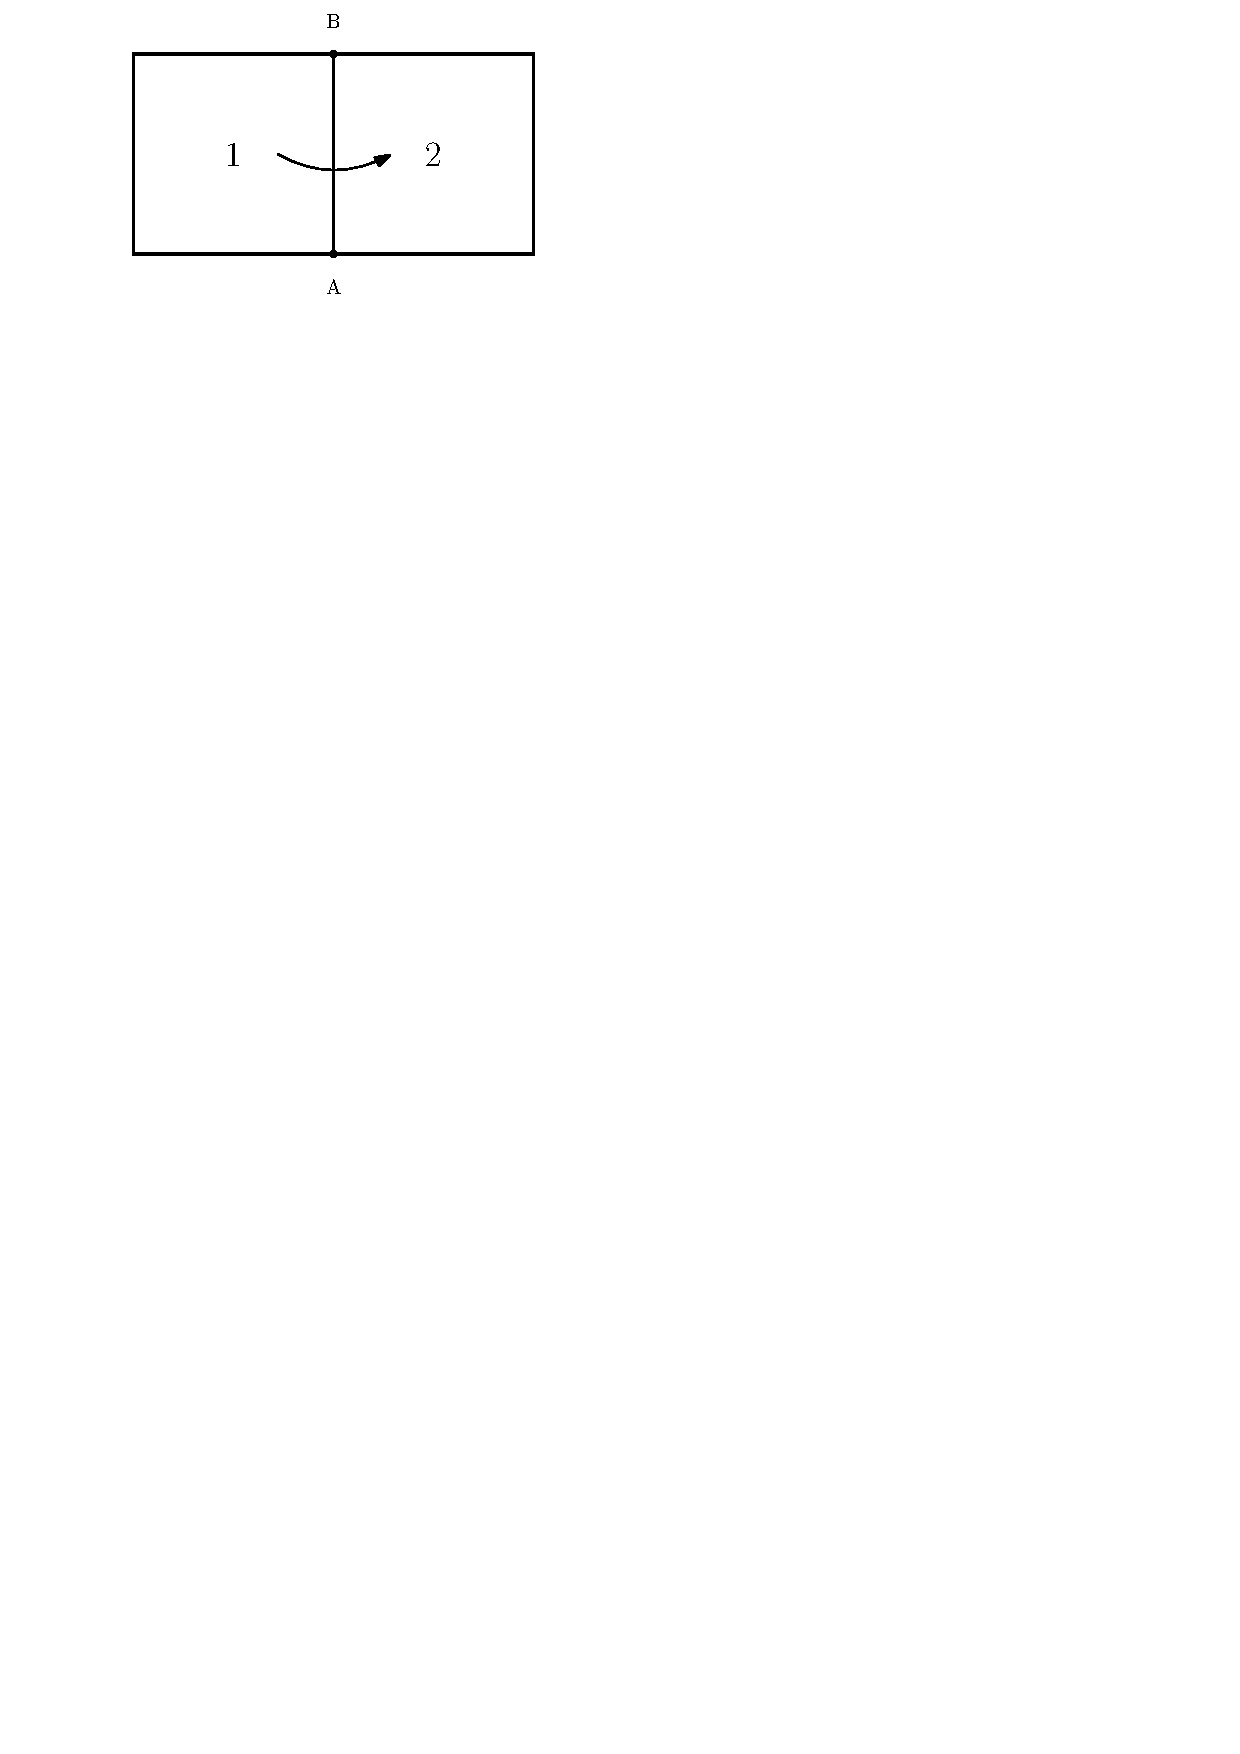
\includegraphics[scale=0.5]{./1.5 Forze e sforzi/1.5-2}
		\centering
		\caption{Si consideri un volume di controllo diviso in due parti}
	\end{figure}
%
Vi è un flusso di quantità di moto dal volume $V_1$ al volume $V_2$, che rappresenta la forza che $V_1$ esercita su $V_2$
	\begin{equation*}
		\int_{AB} \uuline{J}_Q \vdot \uline{n} \dd{S} = \uline{F}_{12}
	\end{equation*}
Ovviamente la quantità di moto nel volume 1 diminuisce della stessa quantità di cui aumenta la quantità di moto nel volume 2.
Dato che a differenza dei solidi si usa la convenzione della normale esterna, rispetto al tensore degli sforzi $T$ della meccanica dei solidi\footnote{in cui per convenzione sono gli sforzi di trazione ad essere positivi} si ha che:
	\begin{equation*}
		\uuline{T} = - \uuline{J}_Q 
	\end{equation*}
È inoltre interessante notare che nella meccanica dei solidi questo ragionamento viene fatto ``al contrario'': si definisce la forza che una parte di solido esercita sull'altra, la si valuta tramite un integrale e l'integrando è il tensore degli sforzi (ed è un tensore per via del tetraedro di Cauchy).
%
\subsection*{Bibliografia 1.5}
\cite[Cap.\ 1.6]{LuchiniQuadrio}\\
\cite[Cap.\ 2.6, 2.9, 2.13]{PnueliGutfinger}